\section{Feistel}

	\begin{frame}
		\begin{center}
			\LARGE{\textcolor{blue}{Cifrari di Feistel}}
		\end{center}
	\end{frame}
	
	\subsection{Substitution Permutation Network (SPN)}
	
	\begin{frame}
		\frametitle{SPN}		
		\begin{itemize}
			\item Eliminare la regolarità statistica $\Leftrightarrow$ Prendere blocchi grandi (64 bit)
			\item Blocchi più grandi $\Rightarrow$ La chiave è la permutazione scelta $(nx2^n)$ bit 
			\item Con blocchi di 64 bit si ha una chiave di $\approx 10^{21}$ bit
			\item Shannon prima e Feistel poi propongono le \tblue{Substitution-Permutation Network} un cifrario a blocchi più semplici ma reiterati un certo numero di volte 
		\end{itemize}
	\end{frame}

	\begin{frame}
	\frametitle{SPN}
	{	
		\fontsize{10}{0}	
		\begin{block}{Diffusione}
			Dissipiamo la ridondanza di ogni singola lettera \emph{spalmandola} su tutto il testo cifrato.
			\begin{itemize}
				\item \tblue{Permutazione} delle lettere (o dei bit) del plaintext secondo regole fissate.
				\item \tblue{Combinazione}: ogni lettera (bit) del ciphertext viene fatto dipendere da più lettere (bit) del plaintext
			\end{itemize}
		\end{block}
		\begin{block}{Confusione}
			Fissata la chiave, rende difficile da analizzare le dipendenze tra plaintext e ciphertext. Si ottiene sostituendo gruppi di lettere (bit) con altri, in funzione della chiave.
		\end{block}
	}
	\end{frame}
	
	\subsection{Feistel}
	
	\begin{frame}
		\frametitle{Cifrari di Feistel}		
		\begin{itemize}
			\item \tblue{Horst Feistel} (IBM) descrive nel 1973 la struttura generale di un cifrario basato sulle SPN
			\item Plaintext \tblue{diviso} in due metà di \emph{w} bit ciascuna, $L_0$ e $R_0$
			\item Ogni metà passa attraverso \emph{n} round tutti con la stessa struttura ma che utilizzano \emph{n} \tblue{sottochiavi} diverse
		\end{itemize}
	\end{frame}

	\begin{frame}
		\frametitle{Schema}
		\begin{columns}
			\begin{column}{0.4\textwidth}
				\begin{center}
					\begin{figure}
						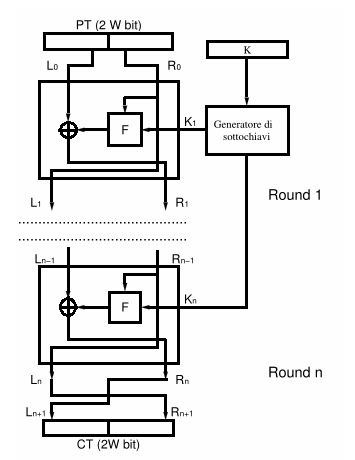
\includegraphics[width=\columnwidth]{img/feistel1}
						\caption{Encryption}			
					\end{figure}
				\end{center}
			\end{column}
			\begin{column}{0.7\textwidth}
				Il generico round $i-esimo$ di encryption può essere descritto come segue:
				$$Round(L_{i-1},R_{i-1},K_i) = (L_i,R_i)$$dove$$
				\begin{cases}
				L_i = R_{i-1} \\
				R_i = F(R_{i-1},K_i) \oplus L_{i-1}
				\end{cases}$$
			\end{column}
		\end{columns}
	\end{frame}

	\begin{frame}
		\frametitle{Schema}
		\begin{columns}
			\begin{column}{0.4\textwidth}
				\begin{center}
					\begin{figure}
						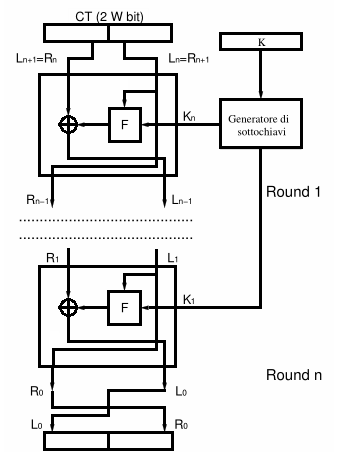
\includegraphics[width=\columnwidth]{img/feistel2}
						\caption{Decryption}			
					\end{figure}
				\end{center}
			\end{column}
			\begin{column}{0.7\textwidth}
				Per la decryption basta far passare il ciphertext dallo \tblue{stesso algoritmo} invertendo l'ordine delle sottochiavi. Infatti
				$$Round(R_{i},L_{i},K_i) = (R_{i-1},L_{i-1})$$ dove
				$$\begin{cases}
				R_{i-1} = L_i \\
				L_{i-1} = R_{i} \oplus F(R_{i-1},K_i) = R_{i} \oplus F(L_i,K_i)
				\end{cases}$$
			\end{column}
		\end{columns}
	\end{frame}

	\begin{frame}
		\frametitle{Cifrari di Feistel}		
		I parametri da scegliere sono quindi:
		\begin{itemize}
			\item Dimensione dei \tblue{blocchi}
			\item Dimensione della \tblue{chiave}
			\item Numero di \tblue{round}
			\item Algoritmo per generare le \tblue{sottochiavi}
			\item Funzione $\tblue{F}$
		\end{itemize}
	\end{frame}

